% Slide illustrations for the OrbitalNet OS deck. One tikzpicture = one PDF page (rasterised by build_deck.py).
% Page order: 1 hero, 2 cnp, 3 enclave, 4 h0, 5 topology, 6 results.  No hand-typed results: see numbers/vars.
\documentclass[tikz,border=0pt]{standalone}
\usepackage[T1]{fontenc}
\usepackage[scaled]{helvet}
\renewcommand{\familydefault}{\sfdefault}
\usepackage{amsmath}
\usetikzlibrary{shadings,arrows.meta,calc,decorations.pathmorphing}
\usepackage{pgfplots}\pgfplotsset{compat=1.17}\usepgfplotslibrary{fillbetween}
% GENERATED by research/figures/paper_main.py -- do not edit
\newcommand{\CausalBugPct}{98\%}
\newcommand{\SimGamma}{0.1}
\newcommand{\SimLengthscale}{1.2}
\newcommand{\SimNEvents}{1000}
\newcommand{\SimNModeled}{587}
\newcommand{\SimNWithheld}{413}
\newcommand{\SimHOneVerdict}{\textbf{fail}}
\newcommand{\SimHTwoVerdict}{\textbf{pass}}
\newcommand{\SimHThreeVerdict}{\textbf{pass}}
\newcommand{\SimTtiP}{23.0\,h}
\newcommand{\SimIdP}{99\%}
\newcommand{\SimTtiBzero}{$>$\,budget}
\newcommand{\SimIdBzero}{48\%}
\newcommand{\SimHolmBzero}{$<10^{-4}$}
\newcommand{\SimRbcBzero}{0.52}
\newcommand{\SimFasterBzero}{50\%}
\newcommand{\SimSlowerBzero}{48\%}
\newcommand{\SimTtiBone}{12.05\,d}
\newcommand{\SimIdBone}{61\%}
\newcommand{\SimHolmBone}{$<10^{-4}$}
\newcommand{\SimRbcBone}{0.63}
\newcommand{\SimFasterBone}{62\%}
\newcommand{\SimSlowerBone}{27\%}
\newcommand{\SimTtiBtwo}{13.8\,h}
\newcommand{\SimIdBtwo}{72\%}
\newcommand{\SimHolmBtwo}{0.00019}
\newcommand{\SimRbcBtwo}{0.19}
\newcommand{\SimFasterBtwo}{30\%}
\newcommand{\SimSlowerBtwo}{49\%}
\newcommand{\SimTtiBthree}{1.59\,d}
\newcommand{\SimIdBthree}{99\%}
\newcommand{\SimHolmBthree}{$<10^{-4}$}
\newcommand{\SimRbcBthree}{0.33}
\newcommand{\SimFasterBthree}{48\%}
\newcommand{\SimSlowerBthree}{25\%}
\newcommand{\SimObsP}{4.2}
\newcommand{\SimObsBthree}{2.9}
\newcommand{\SimHtwoFast}{0.414}
\newcommand{\SimHtwoSlow}{0.152}
\newcommand{\SimHtwoEst}{0.261}
\newcommand{\SimHtwoCI}{[0.153, 0.368]}
\newcommand{\SimHtwoFastCI}{[0.314, 0.514]}
\newcommand{\SimHtwoSlowCI}{[0.113, 0.195]}
\newcommand{\SimTprP}{96\%}
\newcommand{\SimTprBthree}{21\%}
\newcommand{\SimHthreeEst}{76}
\newcommand{\SimHthreeCI}{[66, 84]}
\newcommand{\SimAucP}{0.993}
\newcommand{\SimAucBthree}{0.666}
\newcommand{\SimAucBtwo}{0.696}
\newcommand{\SimAucPown}{0.714}
\newcommand{\SimTprPown}{21\%}
\newcommand{\SimCwWhBthree}{97\%}
\newcommand{\SimCwWhP}{6\%}
\newcommand{\SimAccModP}{100\%}
\newcommand{\SimAccModBthree}{100\%}
\newcommand{\SimFaP}{0\%}
\newcommand{\SimFaPModelError}{13\%}
\newcommand{\SimAccModPModelError}{87\%}
\newcommand{\SimAucPModelError}{0.891}
\newcommand{\SimAucBthreeModelError}{0.706}
\newcommand{\SimAucPCrowding}{0.975}
\newcommand{\SimObsAllP}{4.2}
\newcommand{\SimAccModPAll}{100\%}
\newcommand{\SimCwWhPAll}{6\%}
\newcommand{\SimFlagP}{89\%}
\newcommand{\SimAucAblP}{0.993}
\newcommand{\SimObsAllNoDecay}{3.6}
\newcommand{\SimAccModNoDecayAll}{99\%}
\newcommand{\SimCwWhNoDecayAll}{31\%}
\newcommand{\SimFlagNoDecay}{65\%}
\newcommand{\SimAucAblNoDecay}{0.936}
\newcommand{\SimObsAllNoAdeq}{4.3}
\newcommand{\SimAccModNoAdeqAll}{100\%}
\newcommand{\SimCwWhNoAdeqAll}{6\%}
\newcommand{\SimFlagNoAdeq}{89\%}
\newcommand{\SimAucAblNoAdeq}{0.992}
\newcommand{\SimObsAllBthree}{2.8}
\newcommand{\SimAccModBthreeAll}{100\%}
\newcommand{\SimCwWhBthreeAll}{97\%}
\newcommand{\SimObsAllBtwo}{4.9}
\newcommand{\SimAccModBtwoAll}{88\%}
\newcommand{\SimCwWhBtwoAll}{69\%}
\newcommand{\SimObsAllBone}{3.2}
\newcommand{\SimAccModBoneAll}{80\%}
\newcommand{\SimCwWhBoneAll}{75\%}
\newcommand{\SimObsAllBzero}{5.0}
\newcommand{\SimAccModBzeroAll}{79\%}
\newcommand{\SimCwWhBzeroAll}{1\%}
\newcommand{\SimDeltaKilonova}{1.59}
\newcommand{\SimDeltaShock}{0.32}
\newcommand{\SimDeltaFlare}{-0.56}
\newcommand{\SimDeltaGrb}{0.15}
\newcommand{\SimHtwoModelErrorEst}{-0.098}
\newcommand{\SimHtwoModelErrorCI}{[-0.171, -0.024]}
\newcommand{\SimHtwoCrowdingEst}{0.232}
\newcommand{\SimHthreeModelErrorEst}{17}
\newcommand{\SimHthreeModelErrorCI}{[8, 31]}
\newcommand{\SimAccModBthreeModelError}{99\%}
\newcommand{\SimHOneCrowding}{fail}
\newcommand{\SimHTwoCrowding}{pass}
\newcommand{\SimHThreeCrowding}{pass}
\newcommand{\SimHOneModelError}{fail}
\newcommand{\SimHTwoModelError}{fail}
\newcommand{\SimHThreeModelError}{pass}
\newcommand{\RealCHOneVerdict}{\textbf{pass}}
\newcommand{\RealCHTwoVerdict}{\textbf{pass}}
\newcommand{\RealCHThreeVerdict}{\textbf{pass}}
\newcommand{\RealCHFourVerdict}{\textbf{pass}}
\newcommand{\RealCHFiveVerdict}{\textbf{fail}}
\newcommand{\RealRHOneVerdict}{\textbf{pass}}
\newcommand{\RealRHTwoVerdict}{\textbf{pass}}
\newcommand{\RealRHThreeVerdict}{\textbf{fail}}
\newcommand{\RealRHFourVerdict}{\textbf{pass}}
\newcommand{\RealRHFiveVerdict}{\textbf{fail}}
\newcommand{\RealNEvents}{364}
\newcommand{\RealNWithheld}{88}
\newcommand{\RealNModeled}{276}
\newcommand{\RealCAuc}{0.79--0.81}
\newcommand{\RealCCwWhBthree}{50--56\%}
\newcommand{\RealCAccModBthree}{58--62\%}
\newcommand{\RealCCwWhP}{7--14\%}
\newcommand{\RealCAccModP}{59--63\%}
\newcommand{\RealCCwWhBone}{40--45\%}
\newcommand{\RealCAccModBone}{54--56\%}
\newcommand{\RealCFlagP}{39--47\%}
\newcommand{\RealCFaP}{8\%}
\newcommand{\RealRAuc}{0.77--0.80}
\newcommand{\RealRCwWhBthree}{78--80\%}
\newcommand{\RealRAccModBthree}{59--62\%}
\newcommand{\RealRCwWhP}{12--19\%}
\newcommand{\RealRAccModP}{53--54\%}
\newcommand{\RealRCwWhBone}{48--49\%}
\newcommand{\RealRAccModBone}{51--55\%}
\newcommand{\RealRFlagP}{64--73\%}
\newcommand{\RealRFaP}{24--25\%}
\newcommand{\RealCObsP}{2.3}
\newcommand{\RealCObsBthree}{2.6}
\newcommand{\RealCObsBzero}{5.0}
\newcommand{\RealRObsP}{5.0}
\newcommand{\RealRObsBthree}{5.0}
\newcommand{\RealRObsBzero}{5.0}
\newcommand{\ConfAlpha}{0.1}
\newcommand{\ConfAlphaPct}{10\%}
\newcommand{\ConfLambda}{0.25}
\newcommand{\ConfNFresh}{489}
\newcommand{\ConfNCal}{456}
\newcommand{\ConfHCOneVerdict}{\textbf{pass}}
\newcommand{\ConfHCTwoVerdict}{\textbf{pass}}
\newcommand{\ConfHCThreeVerdict}{\textbf{pass}}
\newcommand{\ConfHCFourVerdict}{\textbf{pass}}
\newcommand{\ConfHCFiveVerdict}{\textbf{pass}}
\newcommand{\ConfHCSixVerdict}{\textbf{fail}}
\newcommand{\ConfFa}{3--6\%}
\newcommand{\ConfAccGain}{6--8~points}
\newcommand{\ConfFlag}{42--55\%}
\newcommand{\ConfAucGain}{+0.012--+0.039}
\newcommand{\ConfAccFreshCL}{66--69\%}
\newcommand{\ConfAccFreshP}{61--66\%}
\newcommand{\ConfAccFreshBthree}{60\%}
\newcommand{\ConfAccFreshBthreeConf}{57--58\%}
\newcommand{\ConfRawFaFreshP}{7--9\%}
\newcommand{\ConfCwUnkCL}{26--32\%}
\newcommand{\ConfCwUnkP}{7--14\%}
\newcommand{\ConfCwUnkBthree}{50--56\%}
\newcommand{\ConfFlagBthreeConf}{41--52\%}
\newcommand{\ConfObsP}{2.3--2.4}
\newcommand{\ConfObsL}{3.1--3.2}

\newcommand{\NSat}{10{,}109}
\newcommand{\vSimAucP}{0.993}
\newcommand{\vSimAucBthree}{0.666}
\newcommand{\vSimTprP}{0.960}
\newcommand{\vSimTprBthree}{0.210}
\newcommand{\vSimCwWhP}{0.060}
\newcommand{\vSimCwWhBthree}{0.970}
\newcommand{\vRealCCwWhP}{0.105}
\newcommand{\vRealCCwWhBthree}{0.530}

\definecolor{navy}{HTML}{0B2545}\definecolor{space}{HTML}{050914}\definecolor{sky}{HTML}{0EA5E9}
\definecolor{cy}{HTML}{22D3EE}\definecolor{amb}{HTML}{F59E0B}\definecolor{grn}{HTML}{16A34A}
\definecolor{rd}{HTML}{DC2626}\definecolor{vio}{HTML}{7C3AED}\definecolor{pale}{HTML}{EEF4FB}
\tikzset{sat/.pic={
    \fill[gray!15,draw=gray!60,line width=.2pt] (-.075,-.06) rectangle (.075,.06);
    \fill[blue!70!cyan,draw=white,line width=.15pt] (-.34,-.05) rectangle (-.11,.05);
    \fill[blue!70!cyan,draw=white,line width=.15pt] (.11,-.05) rectangle (.34,.05);
    \foreach \x in {-.265,-.19,.185,.26} \draw[white,line width=.12pt] (\x,-.05)--(\x,.05);
    \draw[gray!70,line width=.3pt] (-.11,0)--(-.075,0) (.075,0)--(.11,0) (0,.06)--(0,.12);
    \fill[gray!70] (0,.13) circle (.018);}}
\newcommand{\satglow}[3][cy]{\fill[#1,opacity=.18] #2 circle (.28*#3); \fill[#1,opacity=.3] #2 circle (.17*#3); \pic[scale=#3] at #2 {sat};}
\begin{document}
% ═══ 1 HERO 33.867 x 19.05 cm ═══
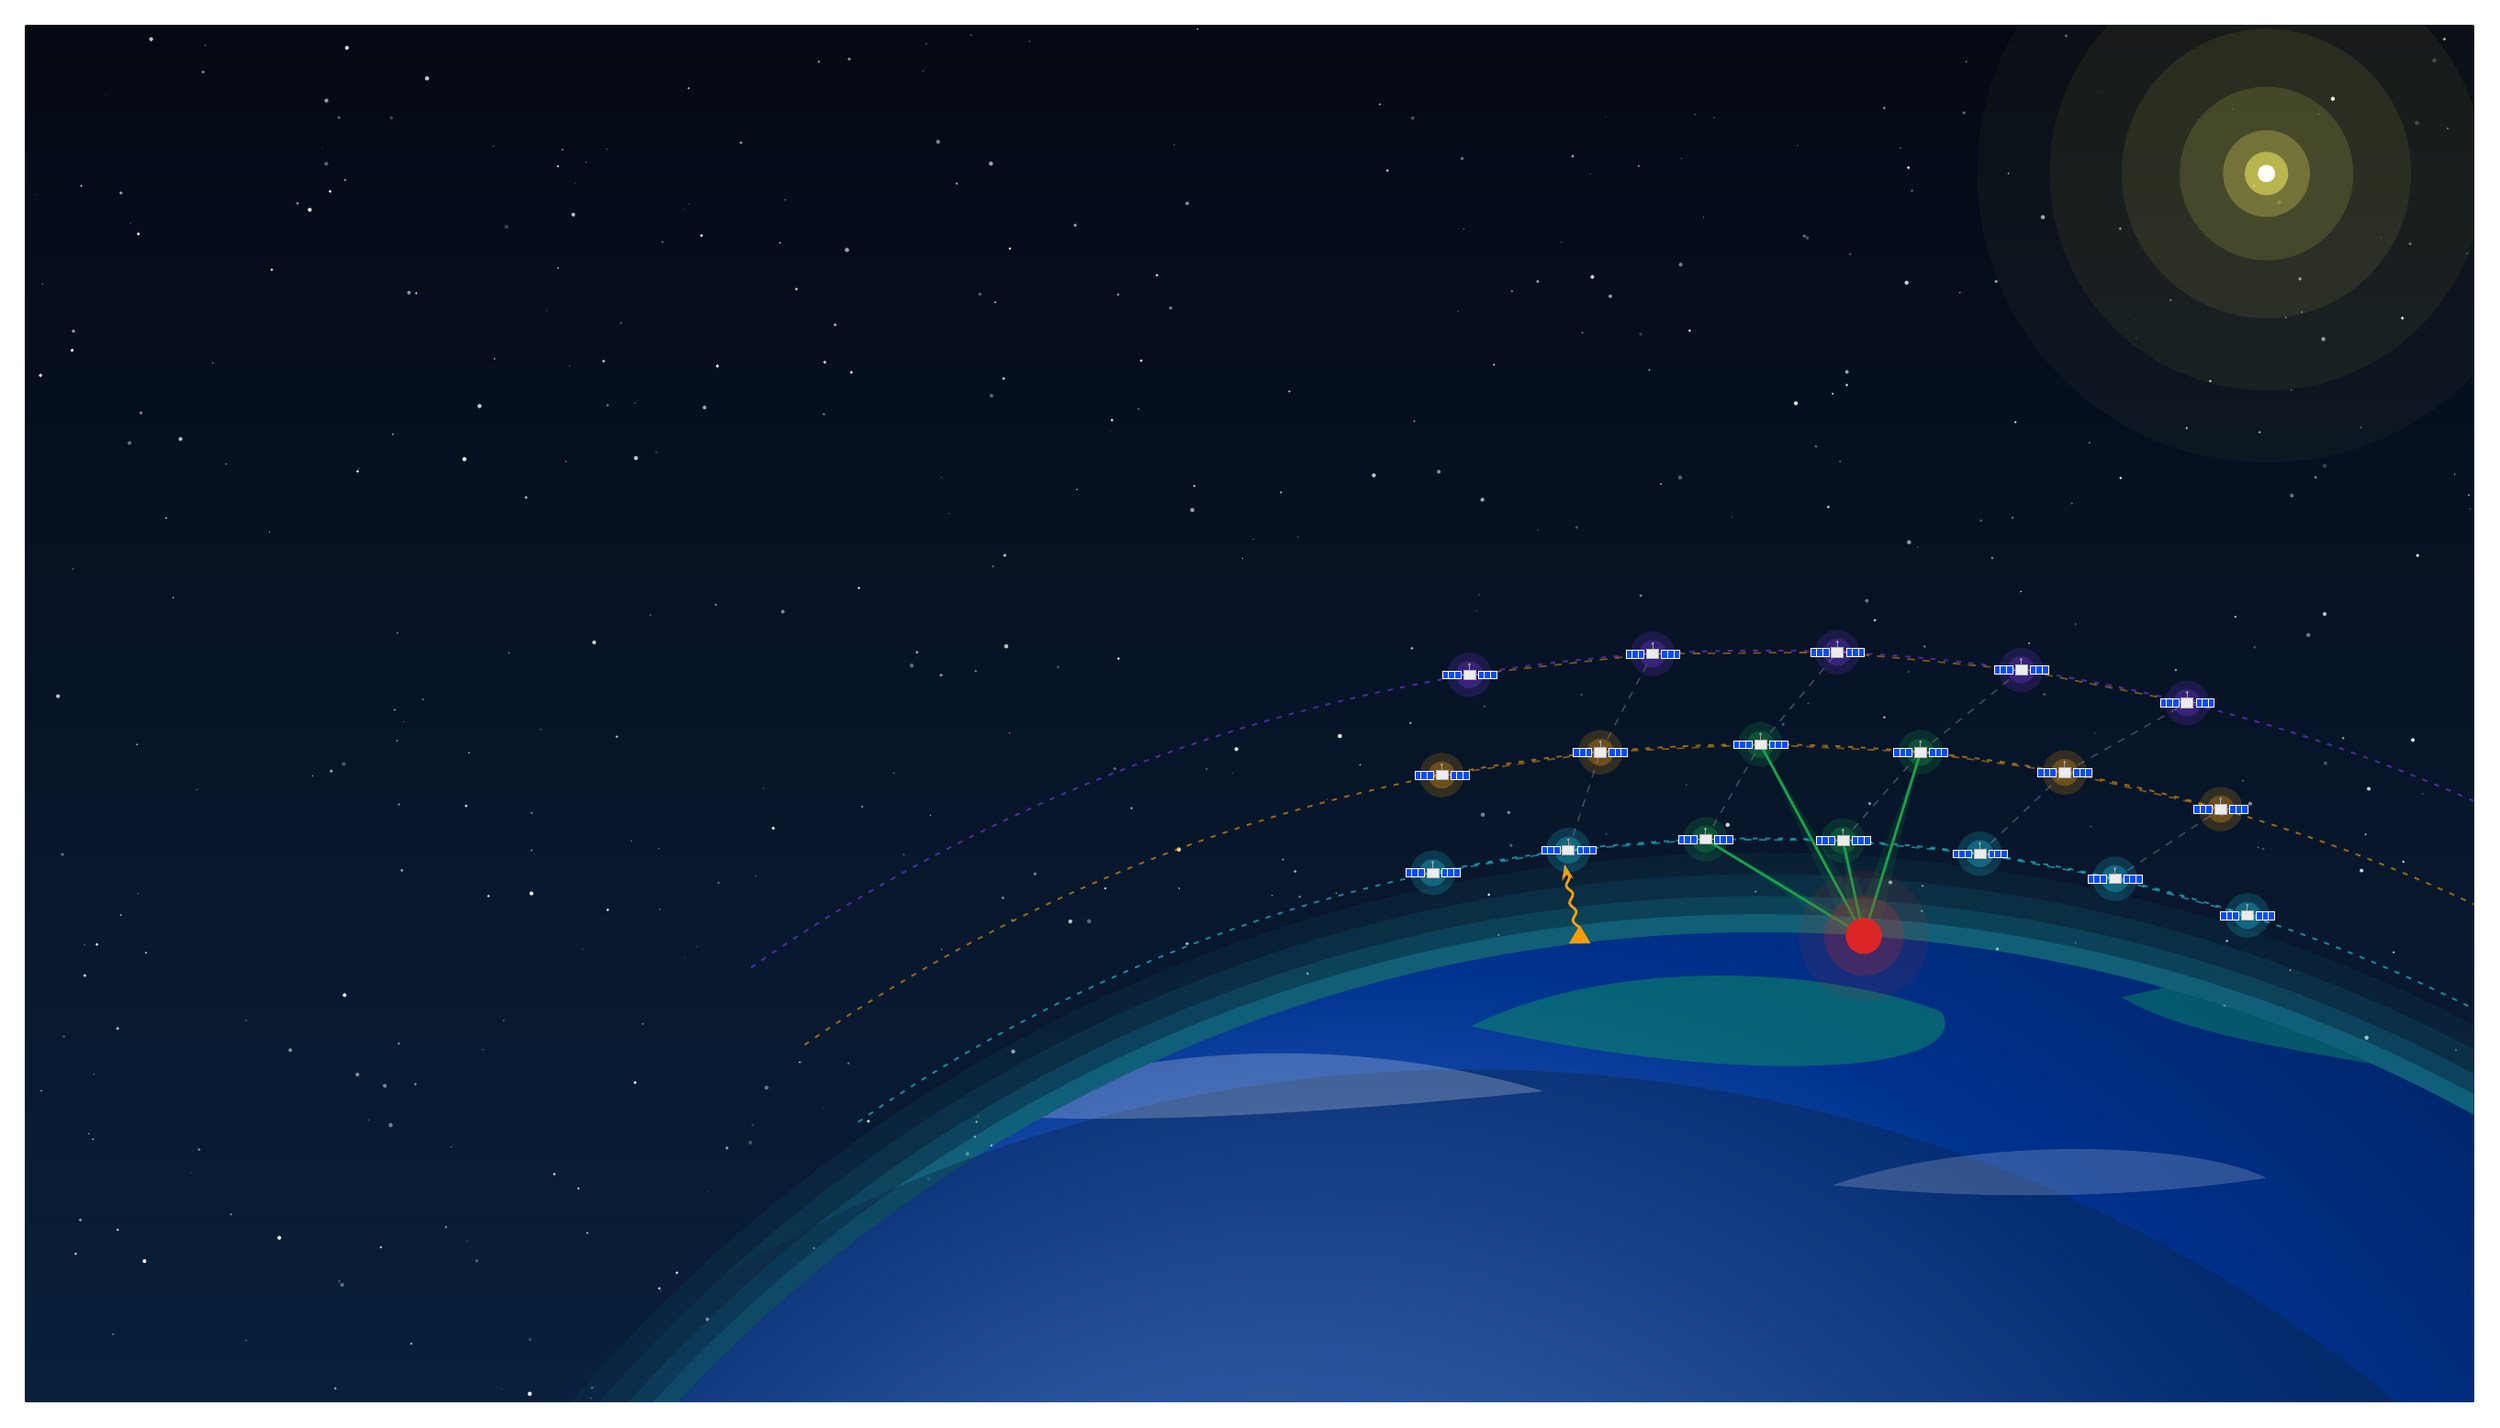
\begin{tikzpicture}
  \clip (0,0) rectangle (33.867,19.05);
  \shade[top color=space,bottom color=navy!85!black] (0,0) rectangle (33.867,19.05);
  \pgfmathsetseed{11}
  \foreach \i in {1,...,520}{\pgfmathsetmacro\o{.2+.75*rnd}\fill[white,opacity=\o] (rnd*33.867,rnd*19.05) circle (.15pt+rnd*.7pt);}
  \foreach \r/\o in {4/.03,3/.05,2/.08,1.2/.13,.6/.25,.3/.5}{\fill[yellow!60!white,opacity=\o] (31,17) circle (\r);}
  \fill[white] (31,17) circle (.12);
  \coordinate (E) at (24,-14);
  \foreach \r/\o in {21.6/.05,21.3/.08,21/.12,20.75/.2}{\fill[cy,opacity=\o] (E) circle (\r);}
  \shade[ball color=blue!65!cyan!80!black] (E) circle (20.5);
  \fill[navy,opacity=.4] ($(E)+(-4,-1.5)$) circle (20.1);
  \begin{scope}\clip (E) circle (20.5);
    \fill[grn!55!teal,opacity=.5] (20,5.2) .. controls (22,6.2) and (25,6) .. (26.5,5.4) .. controls (27,4.6) and (24,4.3) .. (20,5.2);
    \fill[grn!55!teal,opacity=.45] (29,5.6) .. controls (31,6.1) and (33,5.9) .. (34,5.3) -- (34,4.4) .. controls (32,4.8) and (30,5) .. (29,5.6);
    \fill[white,opacity=.22] (13,4) .. controls (16,5.2) and (19,4.9) .. (21,4.3) .. controls (18,4) and (15,3.8) .. (13,4);
    \fill[white,opacity=.18] (25,3) .. controls (27,3.7) and (30,3.6) .. (31,3.1) .. controls (29,2.8) and (27,2.8) .. (25,3);
  \end{scope}
  \foreach \dr/\c in {1.3/cy,2.6/amb,3.9/vio}{\draw[\c,opacity=.6,dash pattern=on 2pt off 3pt,line width=.7pt] (E) ++(55:20.5+\dr) arc (55:125:20.5+\dr);}
  \foreach \n/\a/\dr in {c1/72/1.3,c2/77/1.3,c3/82/1.3,c4/87/1.3,c5/92/1.3,c6/97/1.3,c7/102/1.3,
                         a1/74/2.6,a2/79.5/2.6,a3/84.5/2.6,a4/90/2.6,a5/95.5/2.6,a6/101/2.6,
                         v1/76/3.9,v2/81.5/3.9,v3/87.5/3.9,v4/93.5/3.9,v5/99.5/3.9}{\coordinate (\n) at ($(E)+(\a:20.5+\dr)$);}
  \foreach \p/\q in {c1/c2,c2/c3,c3/c4,c4/c5,c5/c6,c6/c7}{\draw[cy,opacity=.55,line width=.6pt,dashed] (\p)--(\q);}
  \foreach \p/\q in {a1/a2,a2/a3,a3/a4,a4/a5,a5/a6,v1/v2,v2/v3,v3/v4,v4/v5}{\draw[amb,opacity=.5,line width=.6pt,dashed] (\p)--(\q);}
  \foreach \p/\q in {c2/a1,c3/a2,c4/a3,c5/a4,c6/a5,a2/v1,a3/v2,a4/v3,a5/v4}{\draw[white,opacity=.25,line width=.5pt,dashed] (\p)--(\q);}
  \coordinate (T) at ($(E)+(86:20.5)$);
  \foreach \s in {c4,c5,a3,a4}{\fill[grn,opacity=.12] (\s) -- ($(T)+(-.2,0)$) -- ($(T)+(.2,0)$) -- cycle; \draw[grn,line width=1pt] (\s)--(T);}
  \foreach \r/\o in {.9/.1,.55/.22,.25/1}{\fill[rd,opacity=\o] (T) circle (\r);}
  \coordinate (G) at ($(E)+(97:20.5)$);
  \fill[amb] (G) ++(-.15,0) -- ++(.3,0) -- ++(-.15,.25) -- cycle;
  \draw[amb,line width=1pt,-{Stealth[length=6pt]},decorate,decoration={snake,amplitude=1pt,segment length=7pt}] (G) -- ($(c6)+(-.05,-.2)$);
  \foreach \n/\c in {c1/cy,c2/cy,c3/cy,c4/grn,c5/grn,c6/cy,c7/cy,a1/amb,a2/amb,a3/grn,a4/grn,a5/amb,a6/amb,v1/vio,v2/vio,v3/vio,v4/vio,v5/vio}{\satglow[\c]{(\n)}{1.1}}
\end{tikzpicture}
% ═══ 2 CNP message flow ═══
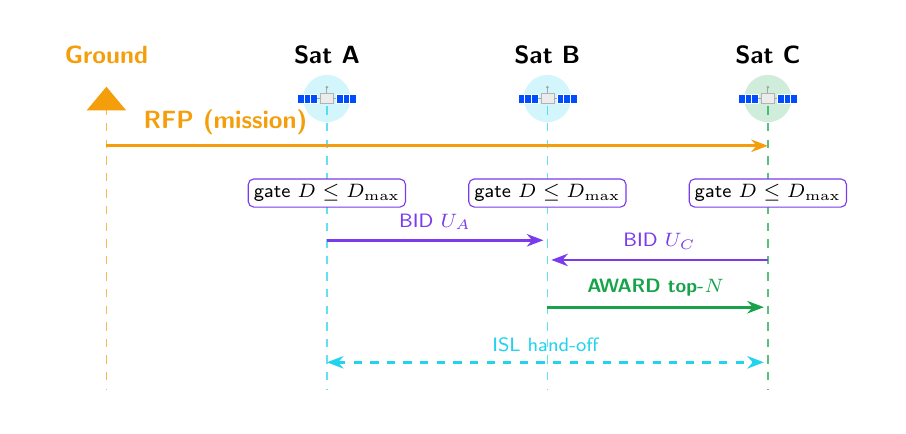
\begin{tikzpicture}[x=1cm,y=1cm,font=\small]
  \fill[white] (-.4,-.5) rectangle (10.4,4.3);
  \foreach \x/\c in {.6/amb,3.4/cy,6.2/cy,9/grn}{\draw[\c!70,dashed,line width=.6pt] (\x,3.3)--(\x,-.3);}
  \fill[amb] (.35,3.25) -- (.85,3.25) -- (.6,3.55) -- cycle; \node at (.6,3.95) {\color{amb}\bfseries Ground};
  \foreach \x/\n/\c in {3.4/A/cy,6.2/B/cy,9/C/grn}{\fill[\c,opacity=.2] (\x,3.4) circle (.3); \pic[scale=1.1] at (\x,3.4) {sat}; \node at (\x,3.95) {\bfseries Sat \n};}
  \draw[amb,-{Stealth[length=6pt]},line width=1pt] (.6,2.8) -- node[above,pos=.18]{\bfseries RFP (mission)} (9,2.8);
  \foreach \x in {3.4,6.2,9}{\node[draw=vio,fill=white,rounded corners=2pt,inner sep=2pt,font=\scriptsize] at (\x,2.2) {gate $D\le D_{\max}$};}
  \draw[vio,-{Stealth[length=6pt]},line width=.9pt] (3.4,1.6) -- node[above,font=\scriptsize]{BID $U_A$} (6.15,1.6);
  \draw[vio,-{Stealth[length=6pt]},line width=.9pt] (9,1.35) -- node[above,font=\scriptsize]{BID $U_C$} (6.25,1.35);
  \draw[grn,-{Stealth[length=6pt]},line width=1.2pt] (6.2,.75) -- node[above,font=\scriptsize\bfseries]{AWARD top-$N$} (8.95,.75);
  \draw[cy,{Stealth[length=6pt]}-{Stealth[length=6pt]},line width=.9pt,dashed] (3.4,.05) -- node[above,font=\scriptsize]{ISL hand-off} (8.95,.05);
\end{tikzpicture}
% ═══ 3 Rolling enclave ═══
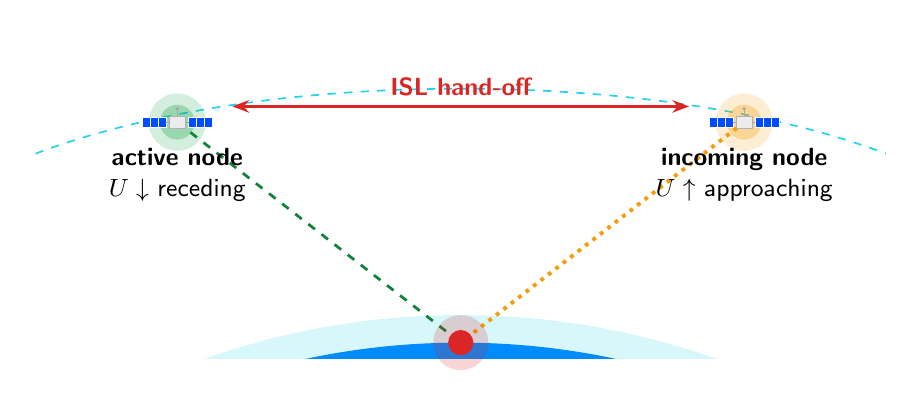
\begin{tikzpicture}[font=\small]
  \begin{scope}\clip (-.5,-.8) rectangle (10.5,3.4);
    \fill[white] (-.5,-.8) rectangle (10.5,3.4);
    \fill[cy,opacity=.18] (5,-10) circle (9.75);
    \shade[top color=blue!45!cyan,bottom color=navy] (5,-10) circle (9.4);
  \end{scope}
  \coordinate (T) at (5,-.6); \coordinate (A) at (1.4,2.2); \coordinate (B) at (8.6,2.2);
  \draw[cy,dashed,line width=.6pt] (-.4,1.8) .. controls (2.5,2.9) and (7.5,2.9) .. (10.4,1.8);
  \draw[grn!80!black,dashed,line width=1pt] (A)--(T); \draw[amb,dotted,line width=1.4pt] (B)--(T);
  \draw[rd,line width=1pt,{Stealth[length=6pt]}-{Stealth[length=6pt]}] ($(A)+(.7,.2)$) -- node[above]{\bfseries ISL hand-off} ($(B)+(-.7,.2)$);
  \satglow[grn]{(A)}{1.3} \satglow[amb]{(B)}{1.3}
  \node[below=6pt,align=center] at (A) {\bfseries active node\\ $U\downarrow$ receding};
  \node[below=6pt,align=center] at (B) {\bfseries incoming node\\ $U\uparrow$ approaching};
  \foreach \r/\o in {.35/.2,.16/1}{\fill[rd,opacity=\o] (T) circle (\r);}
  \node[white,font=\scriptsize\bfseries] at (5,-.15) {TARGET};
\end{tikzpicture}
% ═══ 4 h0 schematic ═══
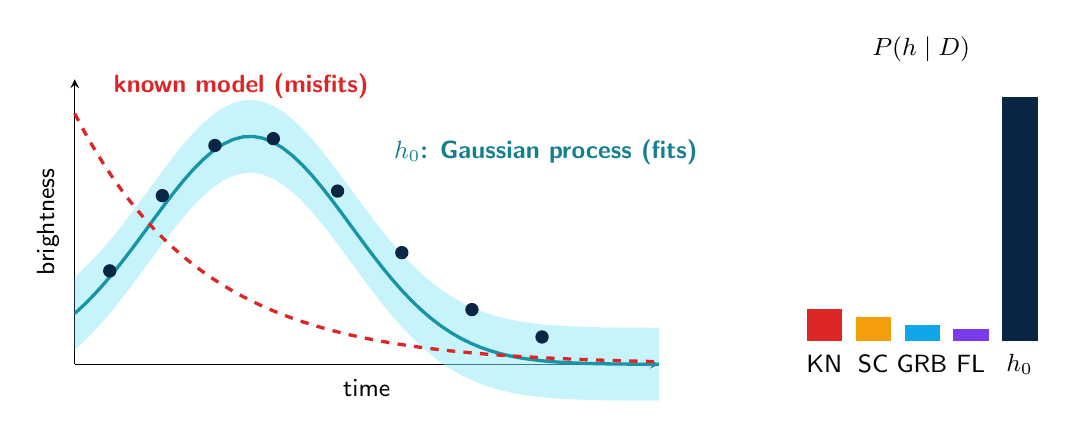
\begin{tikzpicture}
\begin{axis}[width=9cm,height=5.2cm,axis lines=left,xlabel={time},ylabel={brightness},xtick=\empty,ytick=\empty,
  label style={font=\small},xmin=0,xmax=10,ymin=0,ymax=12.5,clip=false]
  \addplot[name path=up,draw=none,domain=0:10,samples=60] {10*exp(-(x-3)^2/6)+1.6};
  \addplot[name path=lo,draw=none,domain=0:10,samples=60] {10*exp(-(x-3)^2/6)-1.6};
  \addplot[cy!50,opacity=.5] fill between[of=up and lo];
  \addplot[cy!70!black,very thick,domain=0:10,samples=60] {10*exp(-(x-3)^2/6)};
  \addplot[rd,very thick,dashed,domain=0:10,samples=60] {11*exp(-x/2.2)};
  \addplot[only marks,mark=*,mark size=2.2pt,navy] coordinates {(.6,4.1)(1.5,7.4)(2.4,9.6)(3.4,9.9)(4.5,7.6)(5.6,4.9)(6.8,2.4)(8,1.2)};
  \node[font=\small\bfseries,rd,anchor=west] at (axis cs:0.5,12.2) {known model (misfits)};
  \node[font=\small\bfseries,cy!60!black,anchor=west] at (axis cs:5.3,9.3) {$h_0$: Gaussian process (fits)};
\end{axis}
\begin{scope}[shift={(9.3,0.3)},font=\small]
  \foreach \i/\h/\l/\c in {0/.4/KN/rd,1/.3/SC/amb,2/.2/GRB/sky,3/.15/FL/vio,4/3.1/$h_0$/navy}{
    \fill[\c] (\i*.62,0) rectangle ++(.45,\h); \node at (\i*.62+.22,-.3) {\l};}
  \node at (1.45,3.7) {\bfseries $P(h\mid D)$};
\end{scope}
\end{tikzpicture}
% ═══ 5 topology ═══
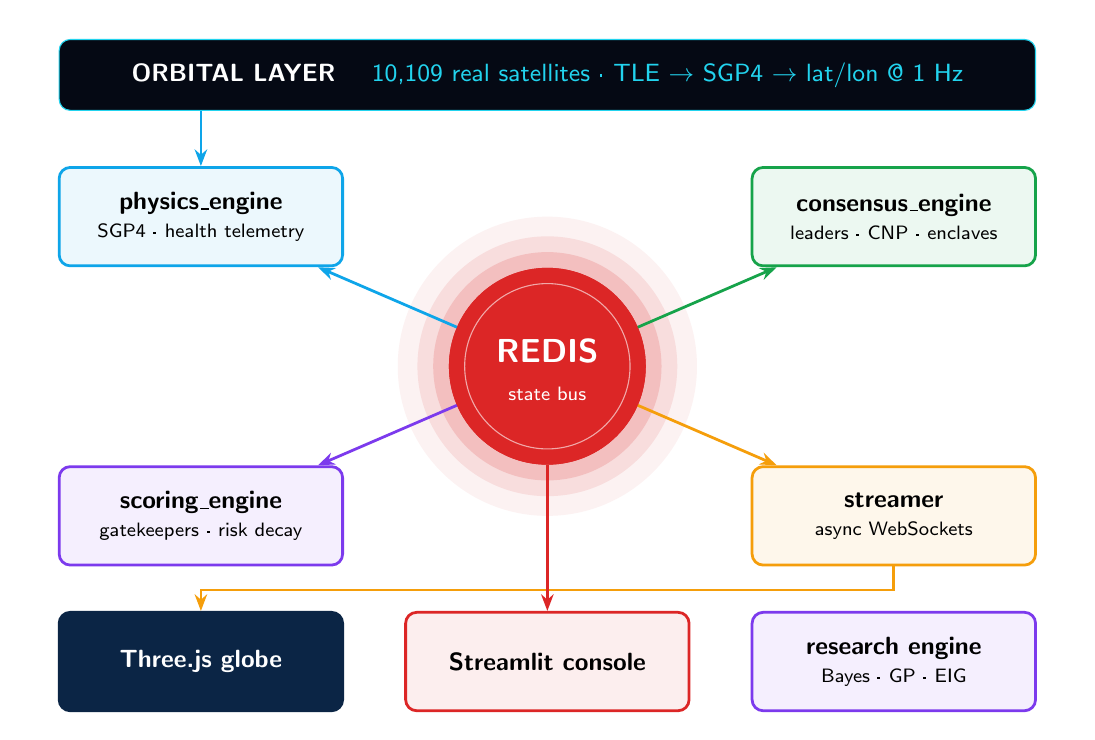
\begin{tikzpicture}[font=\small,
  svc/.style={draw=#1,fill=#1!8,line width=1pt,rounded corners=4pt,minimum width=3.6cm,minimum height=1.25cm,align=center}]
  \fill[white] (-6.6,-4.3) rectangle (6.6,4.3);
  \foreach \r/\o in {1.9/.06,1.65/.1,1.45/.16}{\fill[rd,opacity=\o] (0,0) circle (\r);}
  \fill[rd] (0,0) circle (1.25); \draw[white,opacity=.6] (0,0) circle (1.05);
  \node[white,font=\large\bfseries] at (0,.2) {REDIS}; \node[white,font=\scriptsize] at (0,-.35) {state bus};
  \node[svc=sky] (P) at (-4.4,1.9) {\bfseries physics\_engine\\[-1pt]{\scriptsize SGP4 · health telemetry}};
  \node[svc=vio] (S) at (-4.4,-1.9) {\bfseries scoring\_engine\\[-1pt]{\scriptsize gatekeepers · risk decay}};
  \node[svc=grn] (C) at (4.4,1.9) {\bfseries consensus\_engine\\[-1pt]{\scriptsize leaders · CNP · enclaves}};
  \node[svc=amb] (W) at (4.4,-1.9) {\bfseries streamer\\[-1pt]{\scriptsize async WebSockets}};
  \node[svc=navy,fill=navy,text=white] (G) at (-4.4,-3.75) {\bfseries Three.js globe};
  \node[svc=rd] (U) at (0,-3.75) {\bfseries Streamlit console};
  \node[svc=vio] (R) at (4.4,-3.75) {\bfseries research engine\\[-1pt]{\scriptsize Bayes · GP · EIG}};
  \node[draw=cy,fill=space,text=white,rounded corners=4pt,minimum width=12.4cm,minimum height=.9cm] (O) at (0,3.7)
     {\bfseries ORBITAL LAYER \quad {\mdseries\color{cy} \NSat{} real satellites · TLE $\rightarrow$ SGP4 $\rightarrow$ lat/lon @ 1 Hz}};
  \foreach \n/\c in {P/sky,S/vio,C/grn,W/amb}{\draw[\c,line width=1pt,{Stealth[length=6pt]}-{Stealth[length=6pt]}] (\n) -- (0,0);}
  \draw[sky,line width=1pt,-{Stealth[length=6pt]}] (O.south -| P) -- (P);
  \draw[amb,line width=1pt,-{Stealth[length=6pt]}] (W.south) -- ++(0,-.3) -| (G.north);
  \draw[rd,line width=1pt,-{Stealth[length=6pt]}] (0,-1.25) -- (U);
  \fill[rd] (0,0) circle (1.25); \draw[white,opacity=.6] (0,0) circle (1.05);
  \node[white,font=\large\bfseries] at (0,.2) {REDIS}; \node[white,font=\scriptsize] at (0,-.35) {state bus};
\end{tikzpicture}
% ═══ 6 results ═══
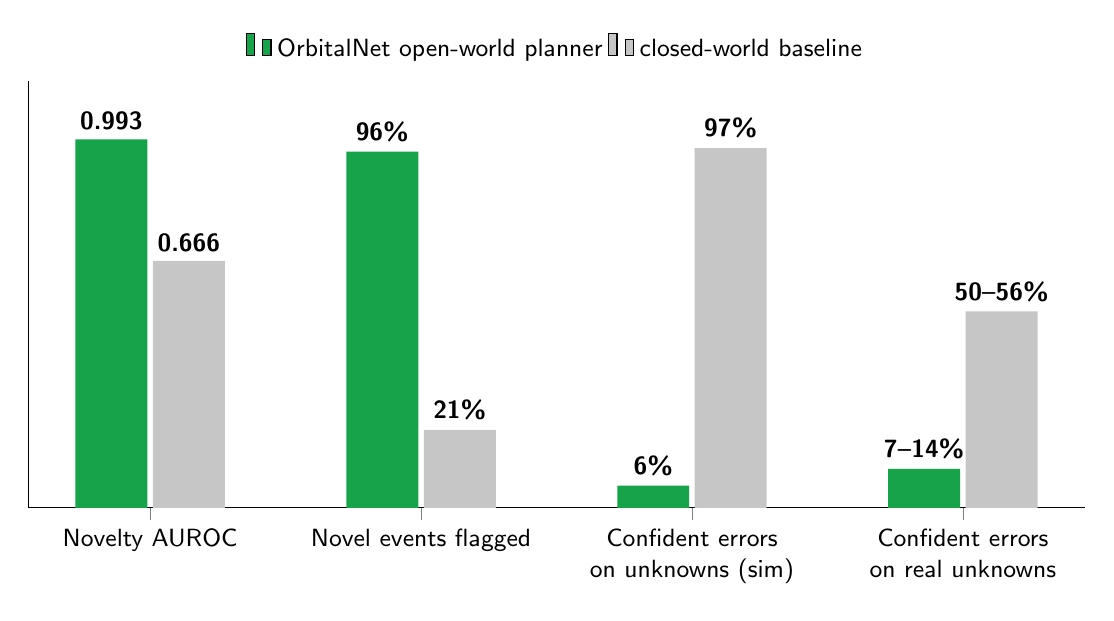
\begin{tikzpicture}
\begin{axis}[ybar,width=15cm,height=7cm,bar width=26pt,ymin=0,ymax=1.15,axis lines*=left,ytick=\empty,
  symbolic x coords={auc,tpr,cw,rcw},xtick=data,enlarge x limits=.15,
  xticklabels={{Novelty AUROC},{Novel events flagged},{Confident errors\\on unknowns (sim)},{Confident errors\\on real unknowns}},
  x tick label style={font=\small,align=center},
  nodes near coords,every node near coord/.append style={font=\small\bfseries},
  legend style={font=\small,draw=none,at={(.5,1.02)},anchor=south,legend columns=2}]
\addplot[fill=grn,draw=none,point meta=explicit symbolic] coordinates
  {(auc,\vSimAucP)[\SimAucP] (tpr,\vSimTprP)[\SimTprP] (cw,\vSimCwWhP)[\SimCwWhP] (rcw,\vRealCCwWhP)[\RealCCwWhP]};
\addplot[fill=gray!45,draw=none,point meta=explicit symbolic] coordinates
  {(auc,\vSimAucBthree)[\SimAucBthree] (tpr,\vSimTprBthree)[\SimTprBthree] (cw,\vSimCwWhBthree)[\SimCwWhBthree] (rcw,\vRealCCwWhBthree)[\RealCCwWhBthree]};
\legend{OrbitalNet open-world planner\quad, closed-world baseline}
\end{axis}
\end{tikzpicture}
\end{document}
